\documentclass[11pt,a4paper]{article}

% For å kunne skrive norske tegn.
\usepackage[utf8]{inputenc}

% \usepackage{minted}

% For å inkludere figurer.
\usepackage{graphicx}

% Ekstra matematikkfunksjoner.
\usepackage{amsmath,amssymb}

%\usepackage[section]{placeins}

% \usepackage{hyperref}
% \hypersetup{%
%   colorlinks=true, % hyperlinks will be black
%   urlcolor=red,
%   linkcolor=red
% }

% For å få tilgang til finere linjer (til bruk i tabeller og slikt).
%\usepackage{booktabs}

% For justering av figurtekst og tabelltekst.
%\usepackage[font=small,labelfont=bf]{caption}

% Subsections A, B,
\renewcommand{\thesection}{\arabic{section}}
\renewcommand{\thesubsection}{\alph{subsection})}

% Disse kommandoene kan gjøre det enklere for LaTeX å plassere figurer og tabeller der du ønsker.
\setcounter{totalnumber}{5}
\renewcommand{\bottomfraction}{0.95}
\renewcommand{\floatpagefraction}{0.35}

\begin{document}

% Rapportens tittel:
\title{Assignment 1: Data Warehousing \\ \large{TDT4300}}
\author{Jonas Myrlund}

% Her ber vi LaTeX om å lage tittelen (til nå har vi bare sagt hva den skal inneholde):
\maketitle

\section{}

\subsection{Explain in your own words the concepts of OLTP (Online Transaction Processing) and OLAP (Online Analytical Processing). Emphasize on the differences between the two concepts in terms of properties and usage.}

OLTP, as the name implies, is used in typical transactional services. In practice, this means many users performing relatively simple updates that require high availability, concurrency, and efficiency. Doing bank transactions, updating customer relations etc. are examples of tasks that involve OLTP.

OLAP is more related to analyzing data. It usually involves a lower volume of transactions, and the queries are often quite complex and involving aggregations. Effectiveness can vary, but it is not unusual for a batch job to take several hours to run.

Moreover, the purposes of the systems differ in themselves: OLTP systems are involved with running the core business, while OLAP systems provide information that is typically used in planning and problem solving activities.

% section sec1 (end)

\subsection{Explain the concept of data cube and the meaning of the term ``cuboids''.}

An $n$-dimensional data cube is the generic $n$-dimensional equivalent of a typical 2-dimensional data table. It embodies the concept of extracting axes from a data set and handling it as a cube of $n$ dimensions.

A cuboid is a possible $n$-dimensional cube that can be extracted from a larger data cube. For an $n$-dimensional data cube there are $2^n$ possible cuboids, ie. the number of possible subsets of the set of dimensions.


\subsection{Explain the data cube operations slice, dice, rollup and drill-down.}

\begin{description}
  \item[Slice] \hfill \\ Picking a subcube by selecting only records sharing one specific value for a chosen dimension.
  \item[Dice] \hfill \\ Slicing with multiple possible values for the chosen dimension.
  \item[Rollup] \hfill \\ Going up the concept hierarchy, broadening the selection.
  \item[Drill-down] \hfill \\ Going down the concept hierarchy, narrowing the selection.
\end{description}

\section{(alternative a)} % (fold)

\subsection{Make a star or snowflake schema for this case description.}

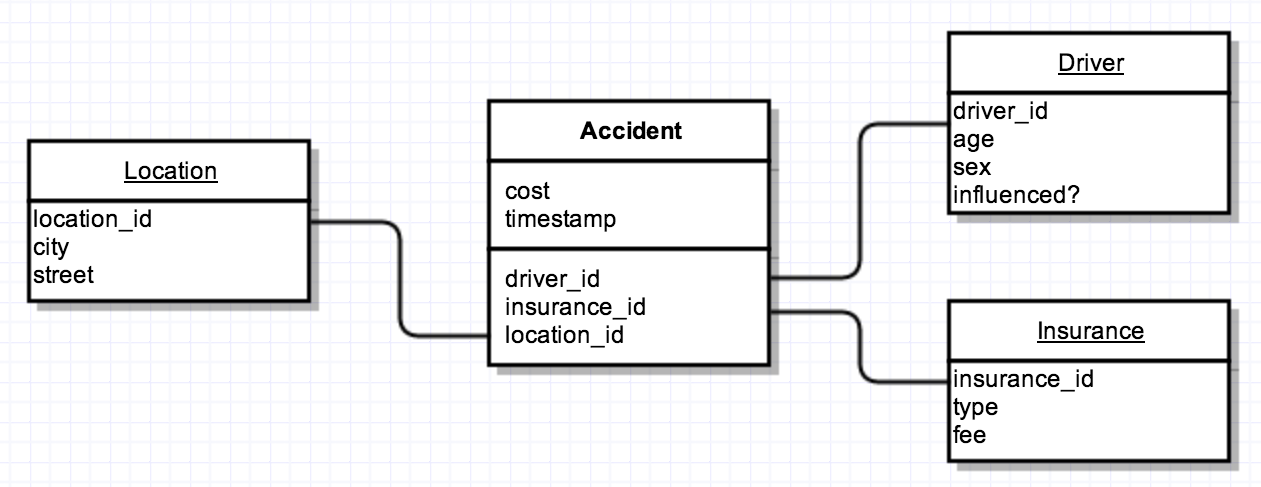
\includegraphics[width=\textwidth]{ex2a}

\subsection{Define two different concept hierarchies (freely chosen dimensions).}

\begin{enumerate}
  \item City $\to$ Street
  \item Year $\to$ Month $\to$ Day (assuming it is extracted as from fact table)
\end{enumerate}

% section sec2 (end)

\section{icCube} % (fold)
\label{sec:iccube}

I created a highly fictuous data set with the turnovers in the bars of Samfundet through January 2014.
It consists of two dimensions: time and location, while the fact table contains the turnovers.

\subsection{Setup in builder}

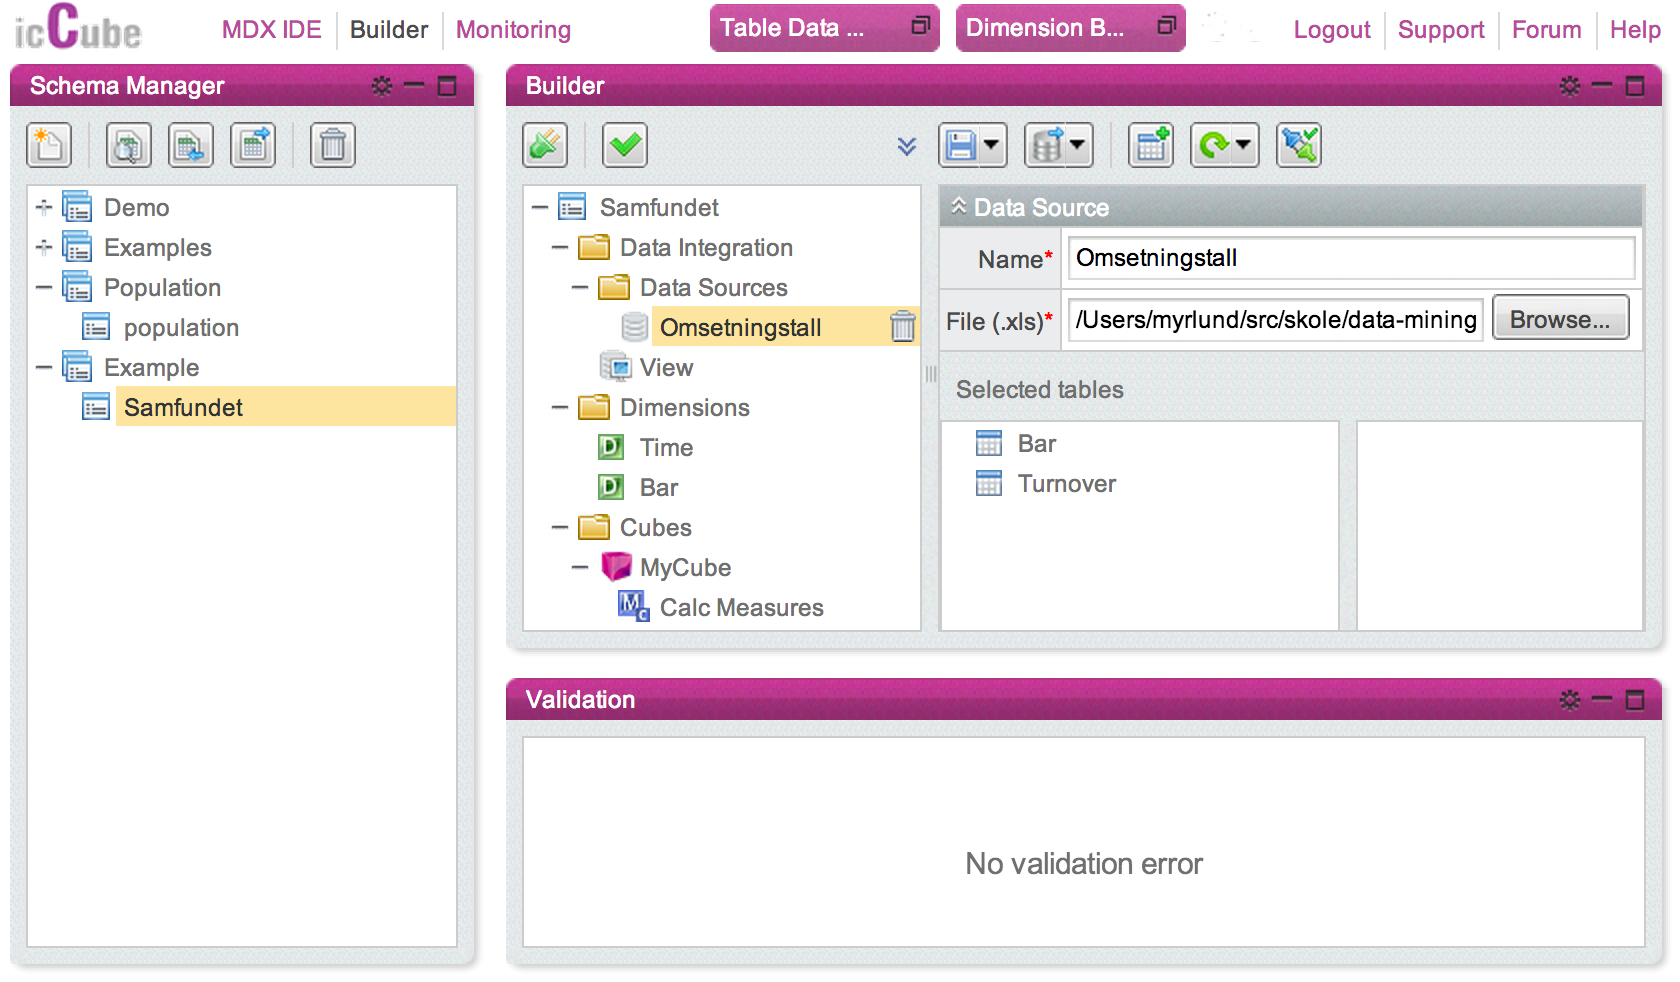
\includegraphics[width=\textwidth]{data_source}

\vspace{2cm}
\noindent

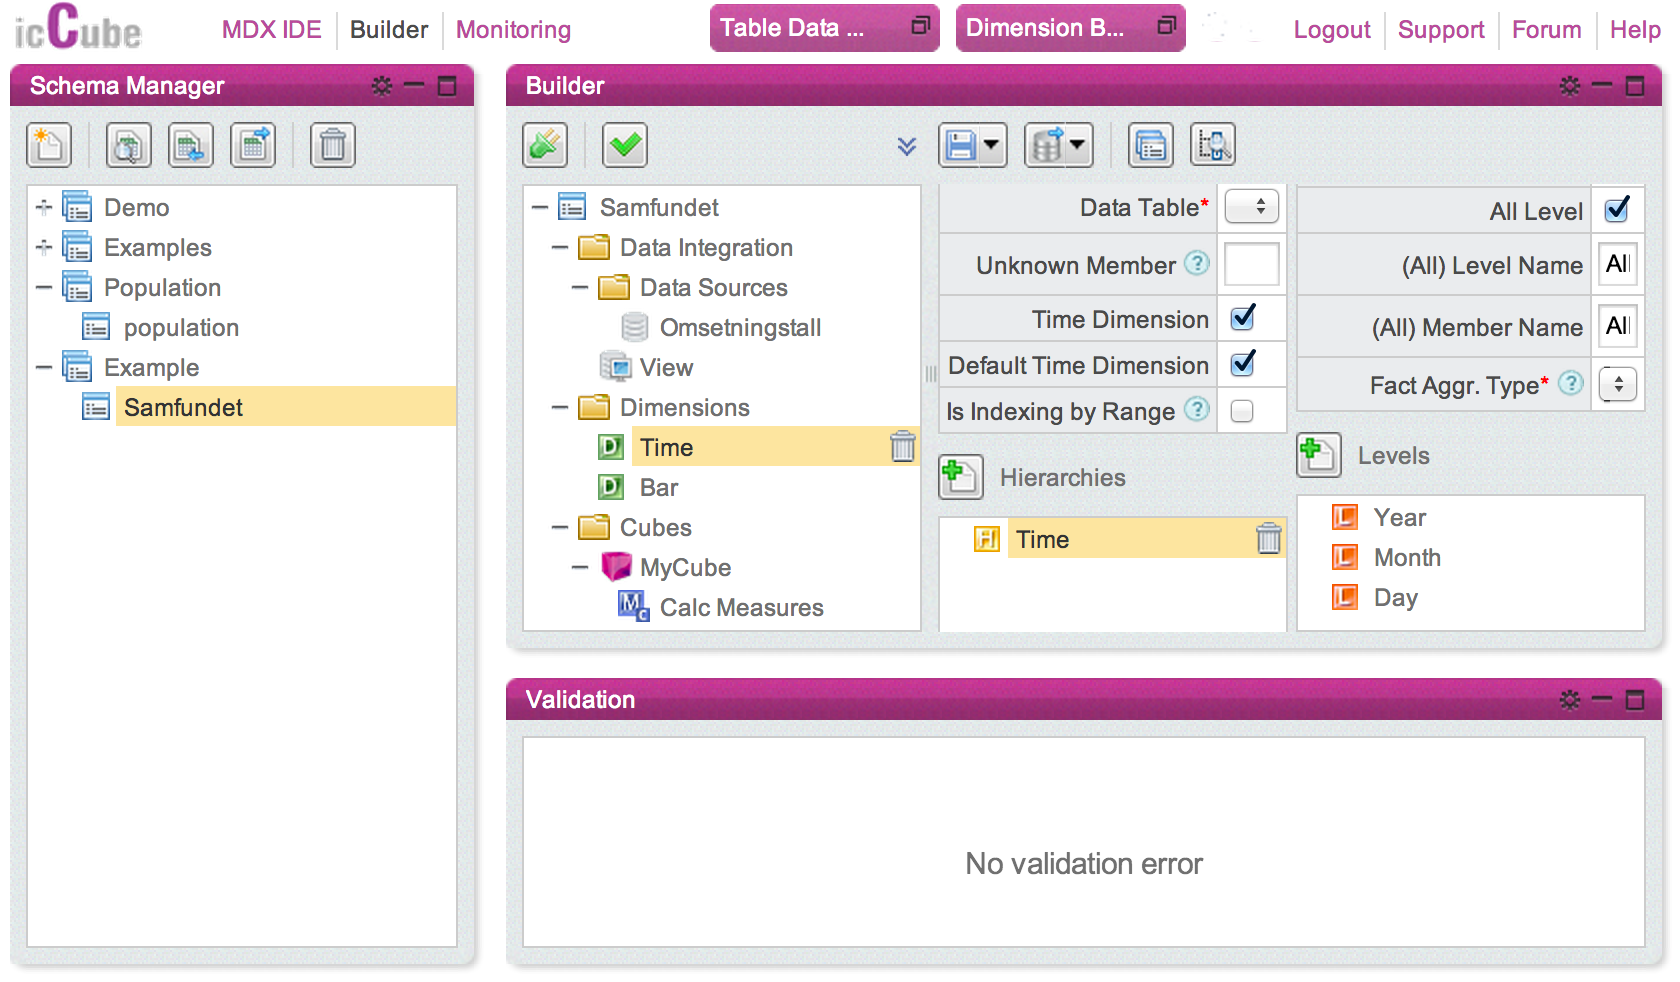
\includegraphics[width=\textwidth]{time_dimension}

\vspace{2cm}
\noindent

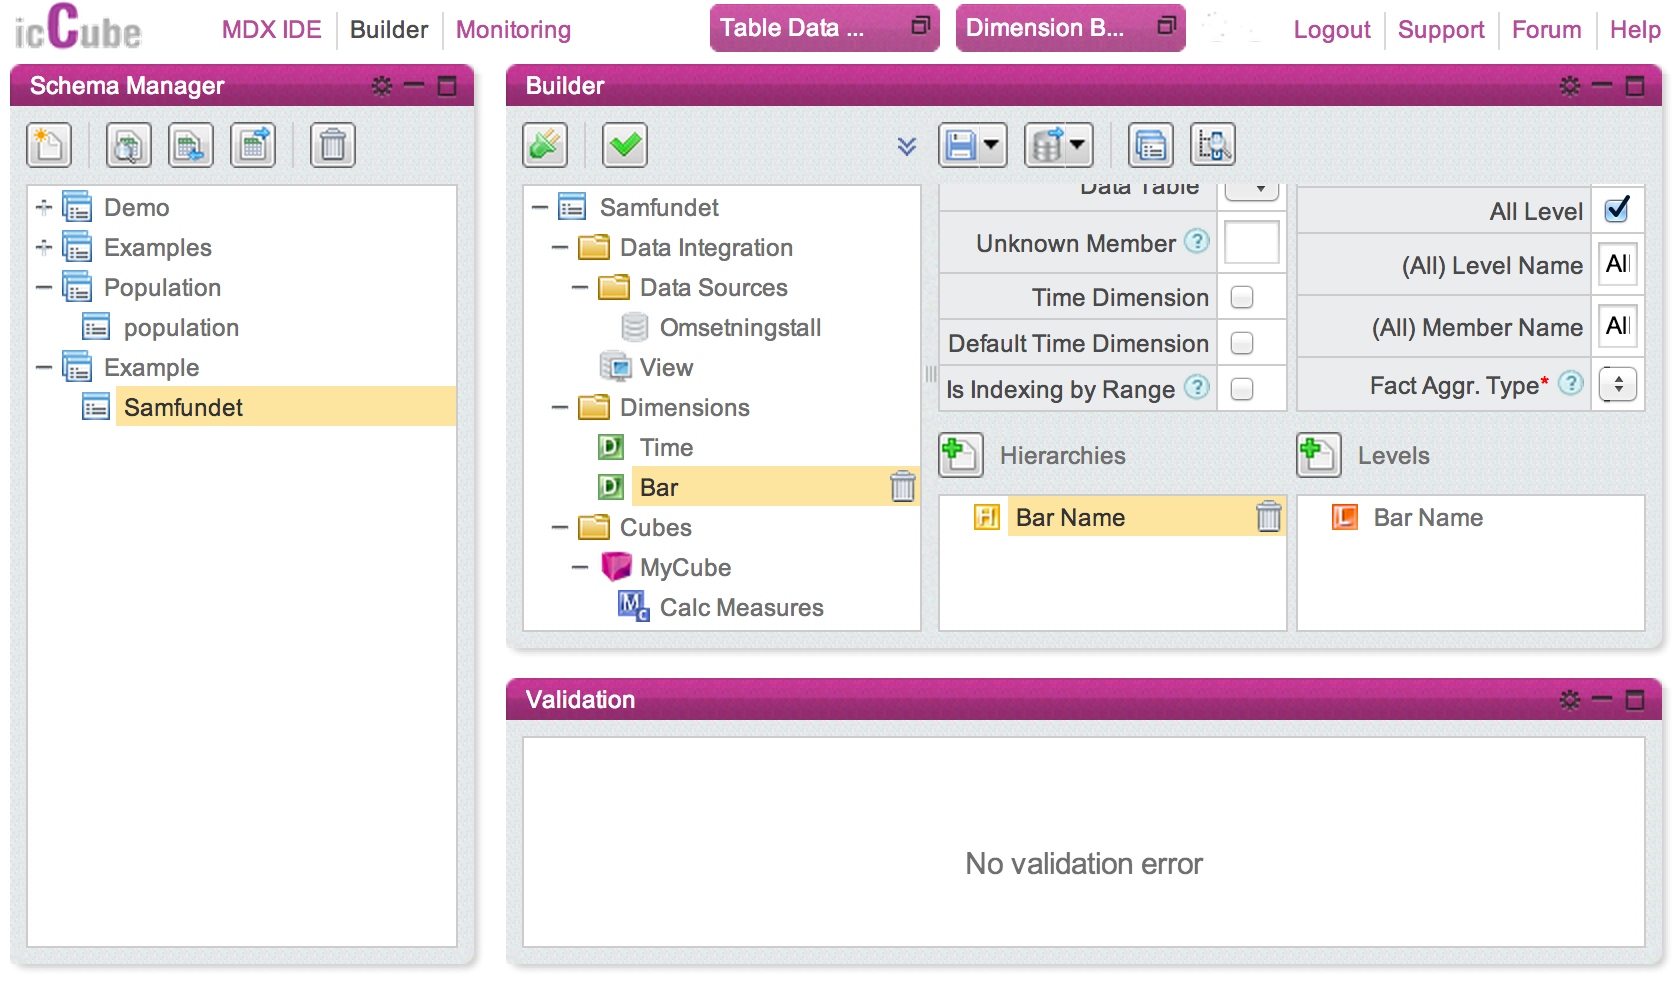
\includegraphics[width=\textwidth]{bar_dimension}

\vspace{2cm}
\noindent

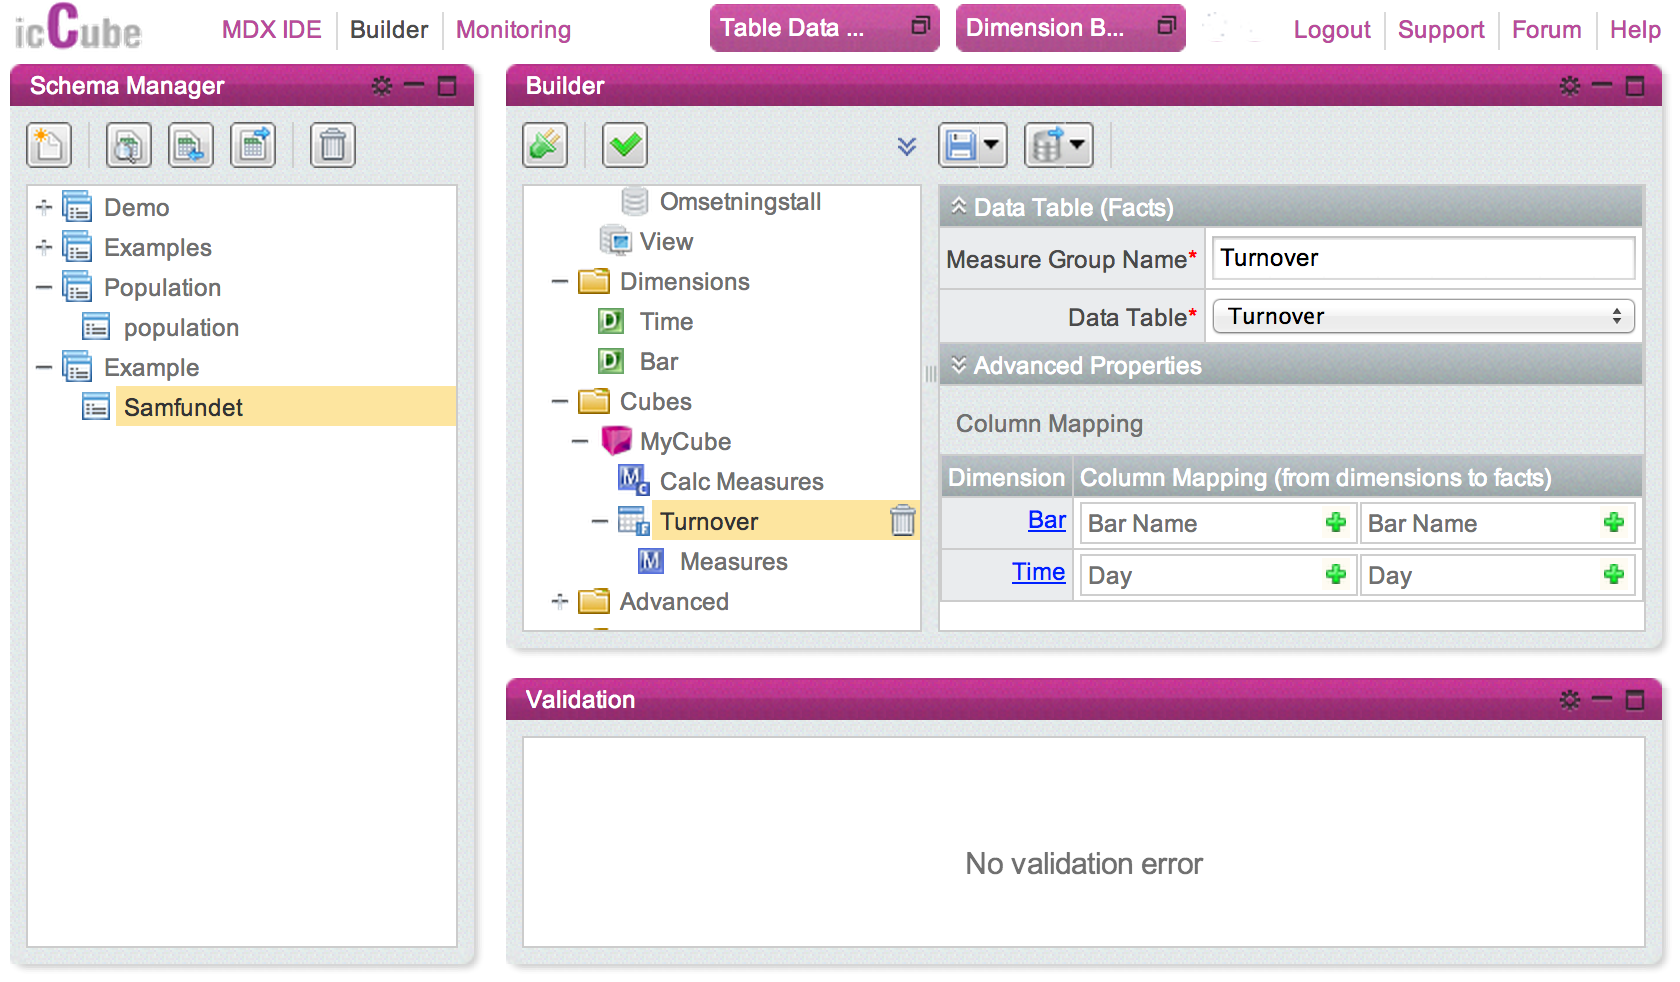
\includegraphics[width=\textwidth]{cube_setup}

\vspace{2cm}
\noindent

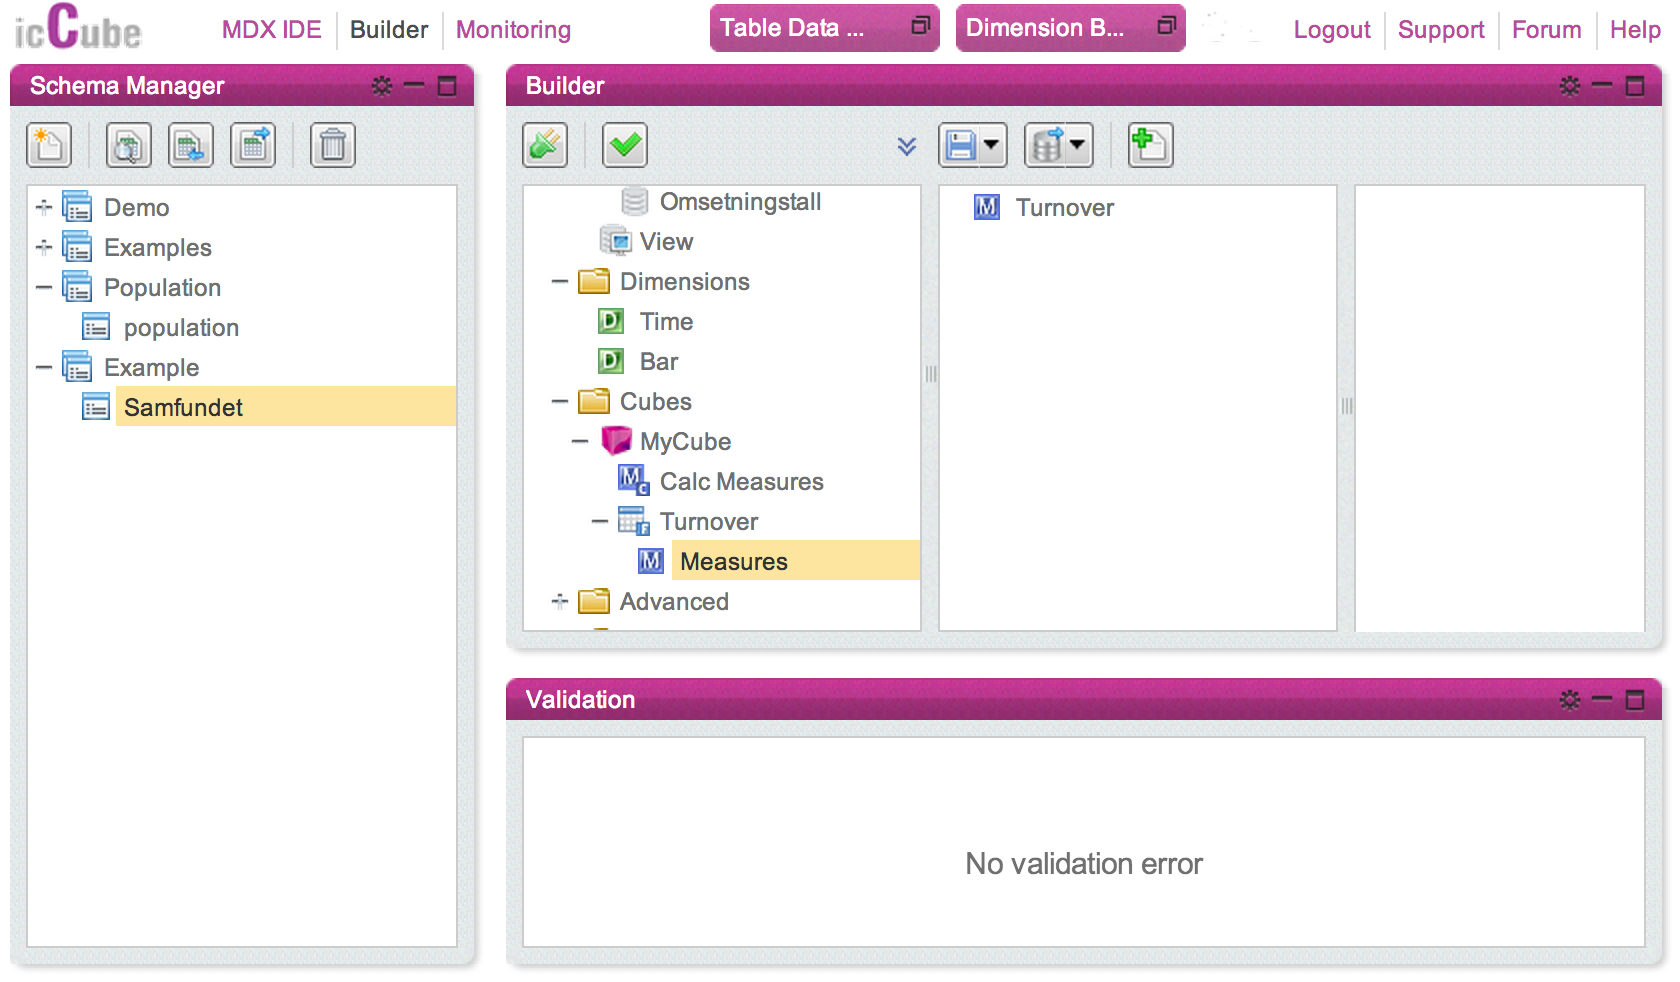
\includegraphics[width=\textwidth]{turnover_measure}

\clearpage
\subsection{Queries}

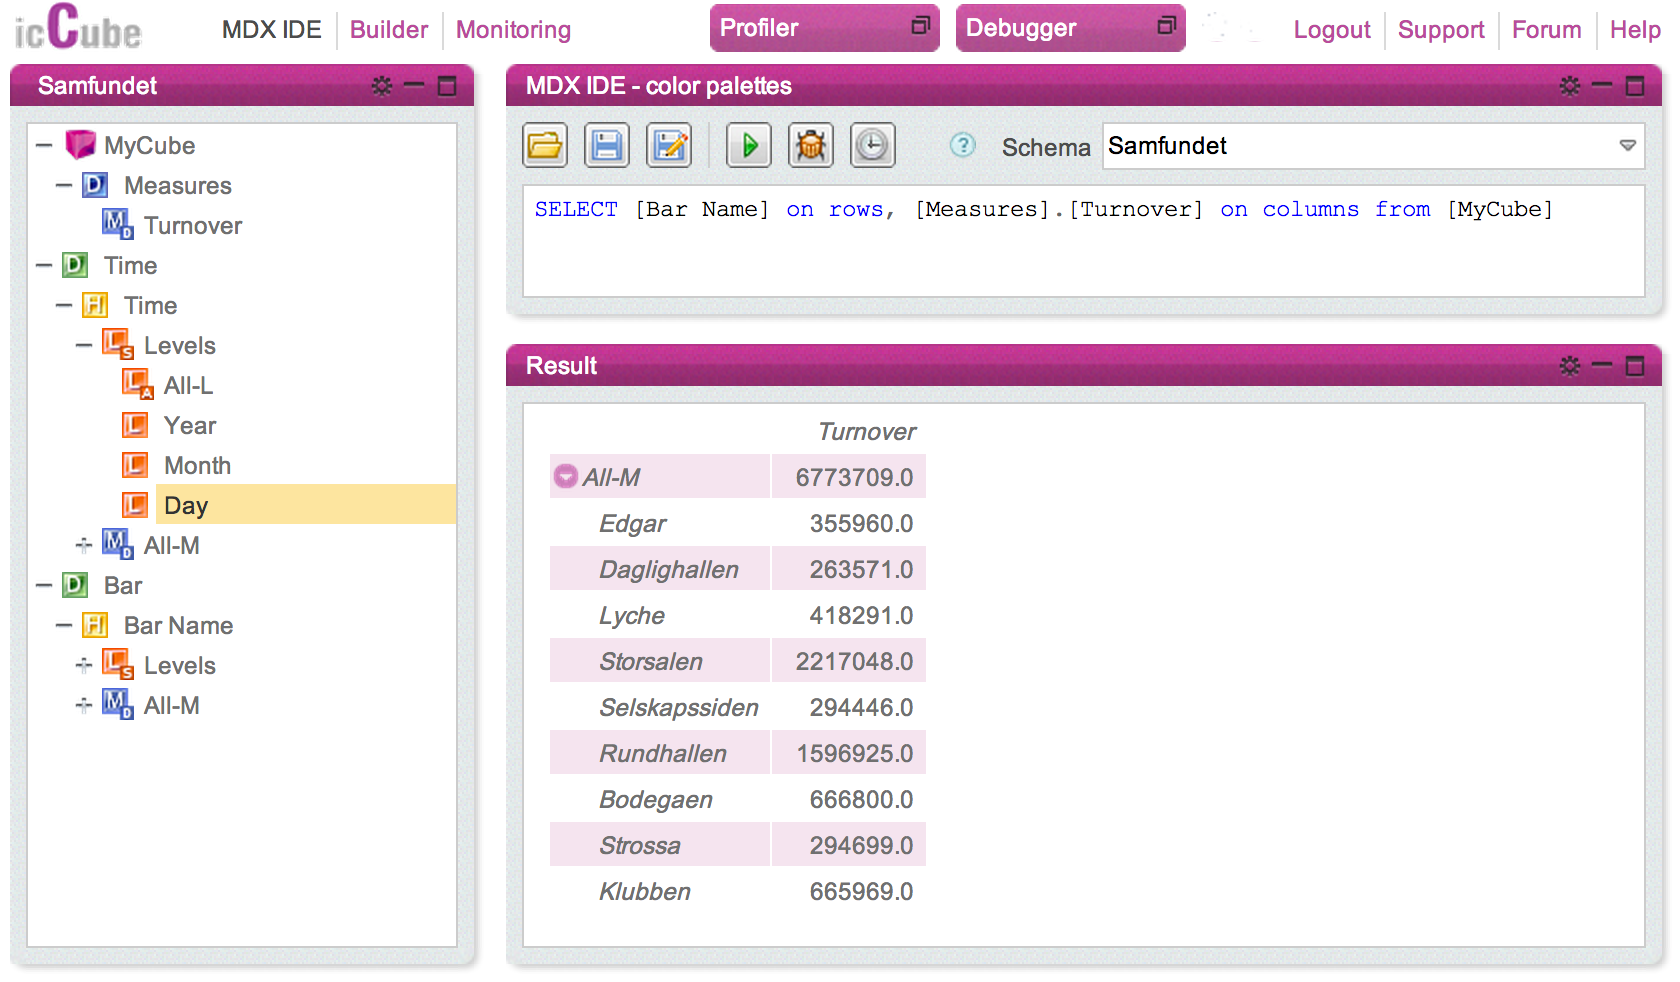
\includegraphics[width=\textwidth]{mdx_query_1}

\vspace{2cm}
\noindent

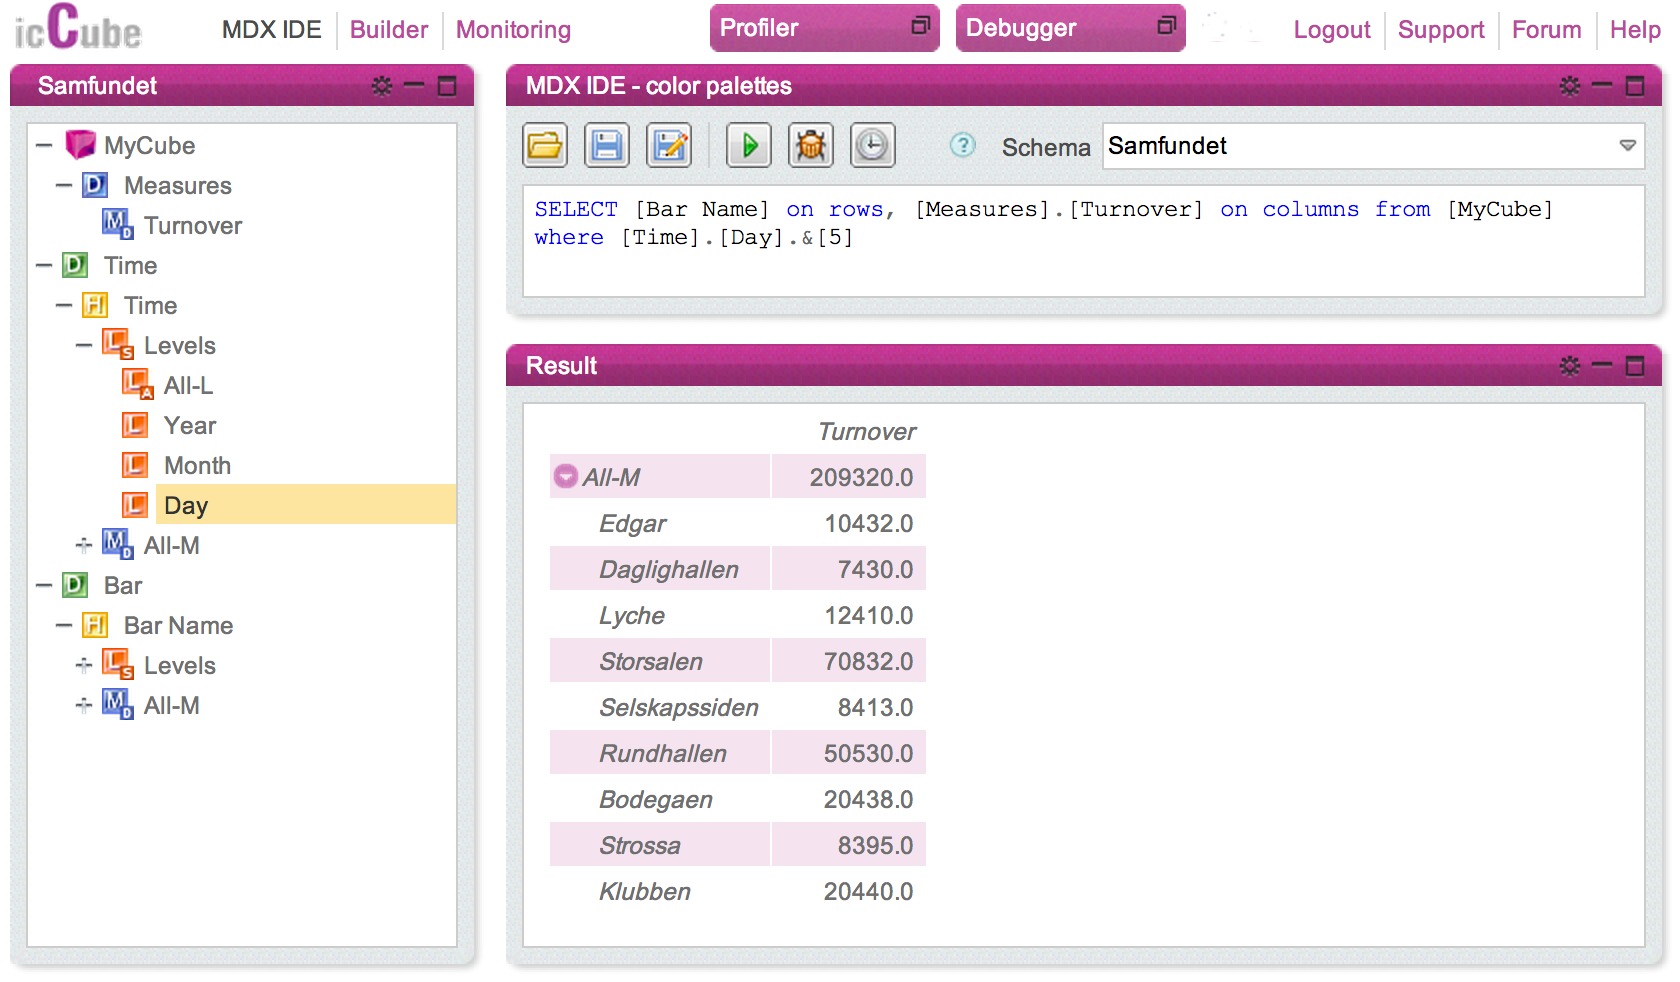
\includegraphics[width=\textwidth]{mdx_query_2}


% section iccube (end)

\end{document}
